\documentclass[11pt]{article}
\usepackage{report}

\title{Solid State Physics \\ Notes}
\author{Jesper Vesterberg (jeve0010@student.umu.se)}

\date{\today}

\begin{document}
\begin{titlepage}
  \maketitle
  \thispagestyle{fancy}
  \lhead{
    Department of physics\\
    Umeå Universitet
  }
  \rhead{\today}
  \begin{abstract}
		Collected notes of the whole course, base primarly on the course material (i.e. hook and halls book ``solid state physics'')
  \end{abstract}
  \cfoot{
    Solid  State Physics\\
  }
\end{titlepage}
\lhead{\theauthor}
\rhead{\thetitle\\\today}
\cfoot{\thepage}


\section{Crystal Structure}
\subsection{Elementary Crystallography}
\subsubsection{The crystal lattice}
The crystal lattice is a way to describe crystal structures. We can take for example graphite as showed in figure \ref {fig:graphite}. In order to create the lattice we take a point in the structure, lets call it $O$ ;), then we need to find all identical positions within the structure .

\begin{figure}[H]
	\centering
	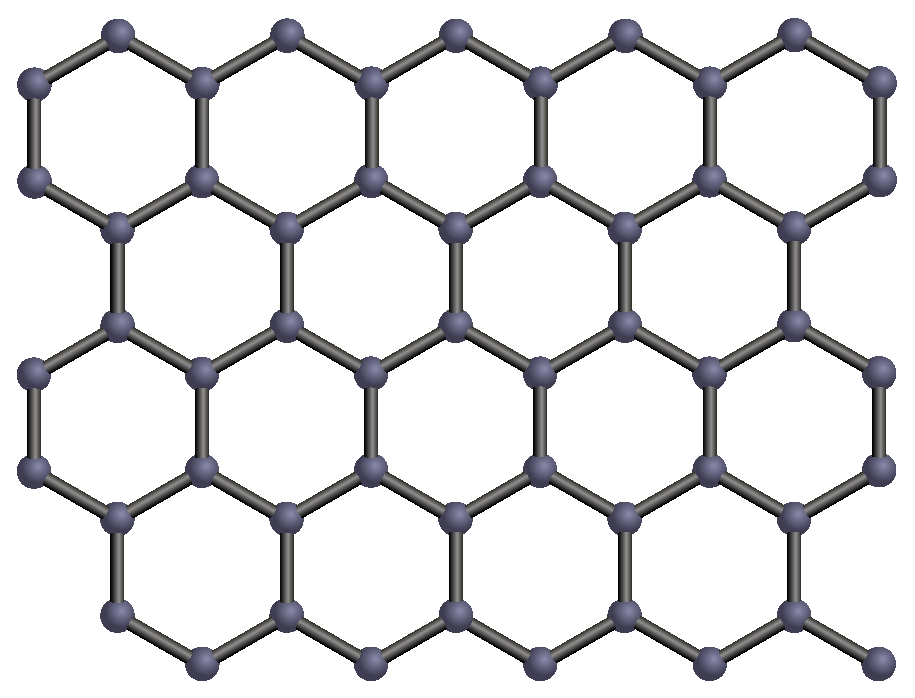
\includegraphics[width=0.8\textwidth]{graphite}
	\caption{Graphite lattice}
	\label{fig:graphite}
\end{figure}

\newpage
This choosing of $O$ and identification of identical position within the structure has been done in figure \ref{fig:graphite-lattice}. Using this lattice which is highlighted in the dotted lines we see we have atoms on all lattice points except the atoms circled in yellow. This actually just fine, this is because we define all atoms related to lattice point through something called the basis, which we will look at in section \ref{sec:basis}, this means that the crystal lattice do not have to coincide with any atom at all. Using the vectors $\mathbf{a}$ and $\mathbf{b}$ here we can define a vector which uniquely defines a point in the lattice relative $O$
\begin{equation}
	\mathbf{r}_{uv }= u\mathbf{a} + v\mathbf{v}
\end{equation}
All points defined through this equation are together called the \textbf{crystal lattice}. An important thing of this lattice is that it possesses \textbf{translational invariance}, which basically means that no matter from what lattice point you're looking at, the structure and environment looks precisely the same. For this to hold we need to presume that the lattice is practically infinite, which is something that is generally true. 

\begin{figure}[H]
	\centering
	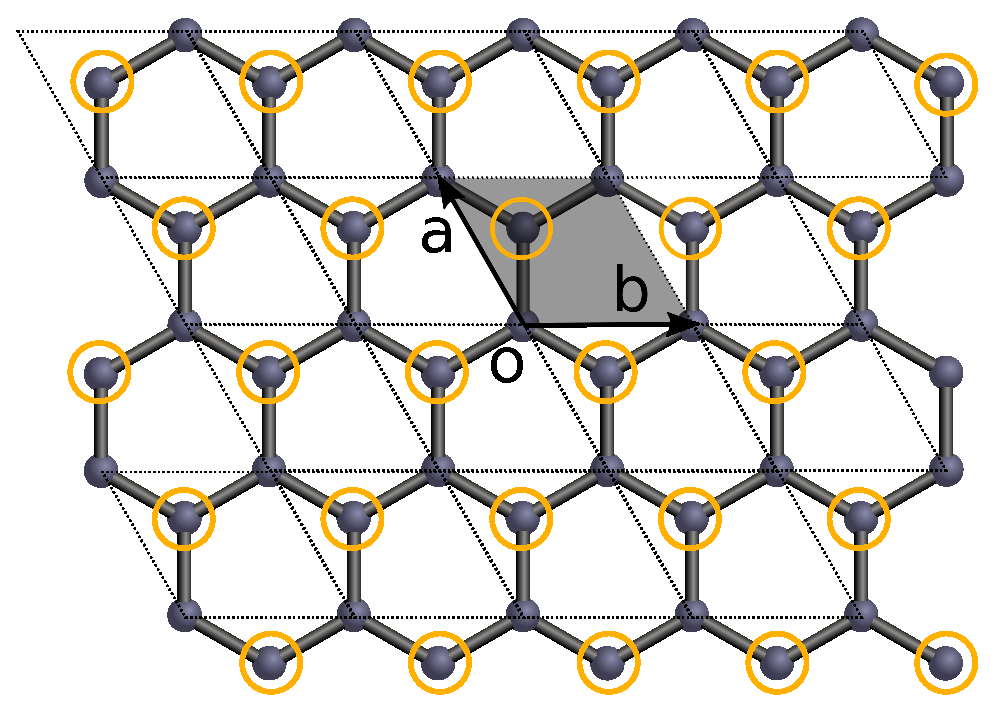
\includegraphics[width=0.8\textwidth]{graphite-lattice}
	\caption{Graphite structure}
	\label{fig:graphite-lattice}
\end{figure}

In three dimension this lattice general arguments extends but the vector that represents all positions in the lattice get an extra term as usual
\begin{equation}
	\mathbf{r}_{uvw} = u\mathbf{a} + v\mathbf{b} + w\mathbf{c}
\end{equation}
and instead of getting an area as covered in grey by $\mathbf{a}$ and $\mathbf{b}$ in figure  \ref{fig:graphite-lattice}, we get a volume, a volume we call the \textbf{unit cell}.

\subsubsection{lattice symmetries}
The lattice symmetries are usually important when looking at the property of a certain solid. In turns out the available possibilities are quite limited too. We lattices such as the \textbf{rectangular lattice}, \textbf{rhombic lattice} and the \textbf{centred rectangular lattice}. Look in the book for further explanation.

\subsubsection{The basis}\label{sec:basis}
The basis is what we use to define a position of a particular atom within a lattice. For our example in figure \ref{fig:graphite-lattice} we have vector 
\begin{equation}
	\mathbf{r}_b = \frac{2}{3}\mathbf{a} + \frac{1}{3} \mathbf{b}
\end{equation}
that defines the position of the yellow circled atom from a lattice point. But the basis also describes the type of atom, thus we end up with the basis 
\begin{equation}
	C(0,0),C(\frac{2}{3}, \frac{1}{3})
\end{equation}
where the first $C$ defines the atom at the lattice point, and the second the other atom which was on on the lattice ($C$ specifies that it is a carbon atom.
Likewise for a three dimensional structure we just add one simple term for the position. 

Taking the symmetry of the basis as well as the crystal lattice, we can sort a crystal into on of the 32 possible \textbf{point symmetry groups} or \textbf{crystal classes} and one of the 230 possible \textbf{space symmetry groups}.

\subsubsection{Crystal planes and directions}
Imagine we have a three dimensional rectangular lattice that we depict in two dimensions as we have done in figure \ref{fig:lattice-planes}. We can then define a multitude of planes that goes through multiple lattice points. In two dimension in looks simply like lines, but if we stretch that out in three dimensions we can easily see the planes, which  is more clearly depicted in figure \ref{fig:lattice-planes-3d}.
\begin{figure}[H]
	\centering
	\includegraphics[width=0.8\textwidth]{lattice-planes}
	\caption{Some lattice planes in the rectangular lattice}
	\label{fig:lattice-planes}
\end{figure}
\begin{figure}[H]
	\centering
	\includegraphics[width=0.8\textwidth]{lattice-planes-3d}
	\caption{Some lattice planes in the rectangular lattice, now in 3D!}
	\label{fig:lattice-planes-3d}
\end{figure}

\newpage
These lattice planes plays an important role in the diffraction of incoming waves (usually light or more generally an electromagnetic wave). Thus it's important to identify different sets. This in done through \textbf{Miller indicies}. These indices are defined through where a plane intersects the crystal axes closest to it's origin, but not through the origin. By looking at figure \ref{fig:lattice-planes-vis} we can see four different examples. if we let $\mathbf{a} = x$, $\mathbf{b}=y$ and $\mathbf{c} =z$ we can see how in (d) how we have a plane that intersects the crystal axes at $(\frac{\mathbf{a}}{1},\frac{\mathbf{b}}{1}, \frac{\mathbf{c}}{3})$. The Miller Indices is then the reciprocal of these factors we multiply the crystal axes with in order to find the intersect point, it's written as $(1 1 2)$. if a plane is parallel to a particular axis it's taken at a zero. 

\begin{figure}[H]
	\centering
	\includegraphics[width=0.8\textwidth]{lattice-planes-vis}
	\caption{Some lattice planes in the rectangular lattice, visually in 3d!}
	\label{fig:lattice-planes-vis}
\end{figure}

\newpage
We should also note that from an atomic view a certain amount of planes could due to symmetry in the crystal lattice be equivalent to eachother. This is depicted in figure \ref{fig:lattice-planes-symmetry}. All these three planes are said to belong to the \textbf{form} $\{100\}$.
\begin{figure}[H]
	\centering
	\includegraphics[width=0.8\textwidth]{lattice-planes-symmetry}
	\caption{These lattice planes is equivalent from an atomic point of view, thus all these three ar written as beloning to the form $\{100\}$}
	\label{fig:lattice-planes-symmetry}
\end{figure}

One often want to specify the directions of a vector $\mathbf{r}$ in a crystal. A vector can be written as 
\begin{equation}
	\mathbf{r} = u\mathbf{a} + v \mathbf{b} + w \mathbf{c}
\end{equation}
We then refer to it as the $[uvw]$ direction. Due to symmetry in cubic crystals the $[uvw]$ direction is actually the normal to the $(uvw)$ plane. It should however be noted that this an exception and only hold for lattices with the symmetries of the cubic lattice.

\subsection{Typical crystal structures}

\begin{figure}[H]
	\centering
	\includegraphics[width=0.8\textwidth]{packed-spheres}
	\caption{packed spheres! in 2d!}
	\label{fig:packed-spheres}
\end{figure}
\subsubsection{Cubic and hexagonal close-packed structures}
\subsubsection{The body-centred cubic structure}
\subsubsection{Structures of ionic solids}



\newpage
\begin{thebibliography}{9}
\end{thebibliography}

\clearpage
\appendix
\section{Appendix}

\end{document}

